% CVPR 2026 Paper Template; see https://github.com/cvpr-org/author-kit
\documentclass[10pt,twocolumn,letterpaper]{article}

%%%%%%%%% PAPER TYPE
\usepackage[pagenumbers]{cvpr} % camera-ready style with page numbers

% Import additional packages in the preamble file, before hyperref
\input{preamble}

\usepackage{graphicx}
\usepackage{amsmath}
\usepackage{amssymb}
\usepackage{booktabs}
\usepackage{multirow}

\definecolor{cvprblue}{rgb}{0.21,0.49,0.74}
\usepackage[pagebackref,breaklinks,colorlinks,allcolors=cvprblue]{hyperref}

% give two-column (figure*) floats more freedom so the results figure fits in body
\renewcommand{\dbltopfraction}{0.92}
\renewcommand{\dblfloatpagefraction}{0.7}
\renewcommand{\topfraction}{0.92}
\renewcommand{\textfraction}{0.07}
\setcounter{dbltopnumber}{2}
\setcounter{topnumber}{3}
\setcounter{totalnumber}{5}

% tighten float/caption spacing to keep the body within four pages
\setlength{\abovecaptionskip}{3pt}
\setlength{\belowcaptionskip}{0pt}
\setlength{\textfloatsep}{8pt plus 2pt minus 2pt}
\setlength{\dbltextfloatsep}{8pt plus 2pt minus 2pt}
\setlength{\floatsep}{6pt plus 2pt minus 2pt}
\setlength{\intextsep}{6pt plus 2pt minus 2pt}

\def\paperID{CS131-2026}
\def\confName{CVPR}
\def\confYear{2026}

%%%%%%%%% TITLE
\title{From Phone Photo to MIDI: A Five-Stage Music Recognition Pipeline\\
and a Study of the Clean-to-Real Domain Gap}

\author{Yameen Sekandari\\
Stanford University\\
CS\,131: Computer Vision, Spring 2026\\
{\tt\small yameen@stanford.edu}
}

\begin{document}
\maketitle

%% abstract
\begin{abstract}
I introduce \emph{antiTranscription}, an end-to-end computer-vision pipeline for
converting a casual smartphone photo of printed sheet music into a playable MIDI
file. My system consists of five learned and traditional steps: (i) a
homography-based perspective rectification using a reliable page-corner cascade;
(ii) Hough-transform staff-line detection coupled with a five-line clustering
algorithm; (iii) morphological staff removal followed by connected-component
symbol segmentation; (iv) a trained convolutional neural network for glyph
recognition, on a $35{,}933$-example crop set derived from the PrIMuS
corpus~\cite{calvo2018primus}; and (v) geometric pitch reading and MIDI
synthesis. I find that the geometry steps are extremely reliable on five real
phone photos (rectification passes on all five with slant below $0.22^{\circ}$;
staff detection on all pages), while my main contribution shows a large
\emph{clean-to-real} domain gap: the classifier that achieves $58.9\%$ on clean
glyphs falls to $22.7\%$ on real-cropped glyphs, a drop of $36.2$ points,
primarily concentrated on delicate symbols like hollow half notes (recognized
with $0\%$ accuracy). This motivates my approach of using a geometry-grounded,
segmentation-free notehead-localization and pitch reader that I show improves
exact pitch accuracy from $14\%$ to $\mathbf{86\%}$ on a test song ($89\%$ within
one step). OMR using geometric reasoning is much more promising for phone images
than an appearance-based classifier trained on clean data.
\end{abstract}

\section{Introduction}
\label{sec:intro}

A huge amount of music is only available as a printed score, rather than a
machine-readable encoding. Optical Music Recognition (OMR)---the automatic
transformation of scanned images of a score into a symbolic form such as MIDI or
MusicXML---can make these works playable, transposable, searchable, and
accessible~\cite{calvo2020understanding}. Although commercial OMR engines excel
at clear scanner output, the most ubiquitous capture device today is the camera
on a phone, which suffers from perspective distortion, varied lighting, shadows,
and sensor noise. This gap between the clean documents upon which OMR engines are
trained and tested, and the messy photos users provide, is, I argue, the primary
reason OMR is not practical.

In this paper, I measure this gap directly. I build \emph{antiTranscription}, a
pipeline that takes a hand-held photo of monophonic printed sheet music taken
with a phone and produces a MIDI file. It includes both geometric vision
components (rectification, Hough staff detection, morphological segmentation,
geometric pitch inference) and a trained convolutional classifier; this allows
me to distinguish those pipeline components which make a smooth transition from
clean to real photographic images from those that do not.

My experiments highlight a stark dichotomy. While my geometric vision stages
perform robustly (all five photos correctly rectified with sub-degree slant, and
every staff detected), my appearance-based classifier decreases from a top
accuracy of $58.9\%$ on clean PrIMuS glyphs~\cite{calvo2018primus} to $22.7\%$ on
crops from real photographs, a drop of $36.2$ points, which is most pronounced on
thin or hollow glyphs. I show that a segmentation-free pitch reader using only
the geometry of noteheads takes advantage of this by achieving $86\%$ accuracy on
a representative piece, compared to the $14\%$ accuracy of the purely
appearance-based approach.

\paragraph{Contributions.}
(i) A complete five-stage phone-photo-to-MIDI pipeline combining classical
geometry with a learned classifier; (ii) a robust rectification cascade and
Hough/clustering staff detector succeeding on $100\%$ of my real test photos;
(iii) a quantified \emph{clean-to-real domain-gap study} for OMR symbol
classification ($58.9\%\!\rightarrow\!22.7\%$) with per-class analysis of where
appearance models break; and (iv) a geometry-grounded, segmentation-free pitch
reader that improves exact pitch accuracy $6\times$ ($14\%\!\rightarrow\!86\%$)
over that baseline. I scope the system to monophonic treble-clef scores without
accidentals or key signatures, isolating perception from full musical parsing.

\section{Related Work}
\label{sec:related}

\paragraph{Classical OMR.}
Classical OMR relies on human-designed stages to perform recognition:
binarization, staff removal and detection, symbol segmentation, and musical
reconstruction~\cite{rebelo2012state,calvo2020understanding}. Staff-line
locations are found with projection profiles, run-length encoding, or Hough
transforms~\cite{duda1972hough} and then removed morphologically, after which
symbols can be detected by connected components~\cite{suzuki1985contours}. My
geometry stages are in this tradition; I have built the pipeline with an
engineered phone-capture correction system, with both a front-end rectification
and a post-pipeline stave confirmation by a spacing-consistency check.

\paragraph{Deep and end-to-end OMR.}
Neural sequence models are recent additions to the OMR literature. Calvo-Zaragoza
and Rizo first developed a full end-to-end monophonic OMR CRNN for the PrIMuS
corpus~\cite{calvo2018primus}; van der Wel and Ullrich propose a convolutional
seq-to-seq model for music transcription~\cite{vanderwel2017seq2seq}; Bar\'o et
al.\ use these ideas for handwritten music notation~\cite{baro2019handwritten};
and glyph-based detectors frame glyph locations as boxes~\cite{pacha2018baseline}.
PrIMuS provides the source for the clean symbols in my training data; I do not
use a full sequence model, instead using a CNN~\cite{lecun1998gradient} for the
discrete pitch-identification task to serve as a controlled probe for how
training from clean symbols transfers to photos.

\paragraph{Domain shift.}
A major topic in vision is overcoming the mismatch between training and
deployment domains through unsupervised domain adaptation~\cite{ganin2015dann},
and in OMR this gap has been addressed by creating synthetically distorted
``camera'' versions of the PrIMuS corpus. I introduce an explicit per-class
quantitative measure of this clean-to-real gap in photos, and demonstrate how my
geometry-based pitch-detection approach largely sidesteps it.

\section{Methodology}
\label{sec:method}

The pipeline consists of five steps. I detail each below, pointing out the
formulas that define its geometry.

\subsection{Perspective Rectification}
\label{sec:method:rectify}
I first warp the phone image to a fronto-parallel view. I binarize the page from
the background using Otsu's method, which finds the threshold $t^\star$ that
maximizes the between-class variance
\begin{equation}
  t^\star = \arg\max_{t}\; \omega_0(t)\,\omega_1(t)\,\big[\mu_0(t)-\mu_1(t)\big]^2,
  \label{eq:otsu}
\end{equation}
where $\omega_i$ and $\mu_i$ represent the probability mass and mean of the two
pixel classes separated by $t$~\cite{otsu1979threshold}. The four corners of the
page are extracted from the page mask via a cascade of increasingly liberal
detectors: intersections between Hough lines~\cite{duda1972hough}, polygonal
approximation of the contours~\cite{suzuki1985contours}, and the minimum-area
bounding rectangle. The first of these to result in a sufficiently large convex
quadrilateral is selected. They determine a $3\times3$ homography $\mathbf{H}$
that transforms any source point $\mathbf{x}=(x,y,1)^\top$ into the rectified
space as
\begin{equation}
  \tilde{\mathbf{x}}' \simeq \mathbf{H}\,\tilde{\mathbf{x}},
  \qquad
  x' = \frac{h_{11}x+h_{12}y+h_{13}}{h_{31}x+h_{32}y+h_{33}},
  \label{eq:homography}
\end{equation}
where $y'$ is defined analogously~\cite{hartley2004multiple}. I check that a
rectification is valid by computing the residual slant of staff lines in the
warped image and by counting the fraction of background pixels which overlap with
the border of the page.

\subsection{Staff Detection}
\label{sec:method:staves}
On the rectified page I use adaptive thresholding and then the Hough line
transform, which allows each edge pixel to vote for the lines that pass through it
\begin{equation}
  \rho = x\cos\theta + y\sin\theta .
  \label{eq:hough}
\end{equation}
Horizontal line candidates ($\theta\approx 90^{\circ}$) are grouped by their
$y$-intercept and combined to form five-line staves. A group of five line
candidates is a stave if the spacing $d_k$ between the $k$-th and $(k{+}1)$-th
line does not vary too much, measured by the coefficient of variation
\begin{equation}
  \mathrm{CV} = \frac{\sigma_d}{\mu_d} < 0.4 .
  \label{eq:cv}
\end{equation}
The average spacing, $s=\mu_d$, provides the fundamental length scale for all
subsequent steps.

\subsection{Staff Removal and Segmentation}
\label{sec:method:segment}
The staff lines are removed by suppressing thin horizontal runs. The gaps this
creates in the note stems are bridged using a vertical morphological closing of
height $\approx s$. Connected components are then extracted as
symbols~\cite{suzuki1985contours}, and rejected if their area, relative to $s^2$,
indicates they are noise.

\subsection{Symbol Classification}
\label{sec:method:cnn}
The $64\times64$ binary images of symbols are passed through \textsc{SymbolCNN},
a four-layer convolution--batchnorm--pooling CNN followed by two fully connected
layers. This is trained using $35{,}933$ crops from PrIMuS~\cite{calvo2018primus},
labelled with nine possible symbols: whole, half, quarter, and eighth notes; four
different rest types; and \emph{other}. Since the classes are not balanced, I
minimize a weighted cross-entropy loss
\begin{equation}
  \mathcal{L} = -\sum_{c} w_c\, y_c \log \hat{y}_c,
  \qquad
  w_c \propto \frac{1}{\sqrt{n_c}},
  \label{eq:wce}
\end{equation}
where $n_c$ is the number of crops in class $c$, which weights the less common
classes more heavily. I assign each crop its correct label based on a strict rule
and discard potentially ambiguous symbol--image pairs.

\subsection{Pitch Inference and a Geometry-Only Reader}
\label{sec:method:pitch}
Given the centroid of a notehead located at pixel $y_{\text{head}}$ and the stave
containing it, whose bottom line is at pixel $y_{\text{bottom}}$, I calculate its
position on the stave (in units of half-spaces)
\begin{equation}
  p = \mathrm{round}\!\left(\frac{y_{\text{bottom}}-y_{\text{head}}}{s/2}\right).
  \label{eq:staffpos}
\end{equation}
I map a position on a treble-clef staff (bottom line E4) to a MIDI number by a
deterministic mapping, and provide the associated note duration as determined by
the classifier.

\paragraph{Geometry-only reader.}
Since I find that classification is the least robust step
(Sec.~\ref{sec:results}), I present a reader that performs segmentation-free pitch
inference. After a preliminary filling-in of noteheads using connected-component
analysis on the background pixels, I locate candidates using normalized
cross-correlation with a synthetic ellipse $T$ of size proportional to $s$
\begin{equation}
  R(u,v) = \frac{\sum_{i,j} \big(I_{u,v}(i,j)-\bar I_{u,v}\big)\big(T(i,j)-\bar T\big)}
                {\sqrt{\sum_{i,j}\big(I_{u,v}(i,j)-\bar I_{u,v}\big)^2\;\sum_{i,j}\big(T(i,j)-\bar T\big)^2}},
  \label{eq:ncc}
\end{equation}
where $I_{u,v}$ refers to the image patch at $(u,v)$ beneath the template.
Candidates at peaks of $R$ are found and their neighbors removed with greedy
non-maximum suppression. I discard detections of time signatures or clef margins,
and I filter rests and stems based on their solidity: candidates that remain
solid under a notehead-sized opening are likely true noteheads. Final candidates
are mapped to their MIDI pitch using Eq.~\eqref{eq:staffpos} and staff-position
information.

\section{Experiments and Results}
\label{sec:results}

\paragraph{Data.} I run the system on five hand-held phone photos of printed
monophonic scores: \emph{Yankee Doodle}, \emph{Twinkle Twinkle}, \emph{Mary Had
a Little Lamb}, a CS\,131 motif, and \emph{London Bridge}. Four images undergo
the whole pipeline; one (\emph{London Bridge}) is a failure case
(Sec.~\ref{sec:results:limits}). For classification I use a mined database of
$35{,}933$ $64\times64$ glyph crops, all sourced from clean PrIMuS, with $20\%$
held out for validation; all pitches were transcribed by hand.

\subsection{Geometry stages are robust}
\label{sec:results:geometry}
Rectification is successful on all five images: the slant on remaining staves is
$\le 0.22^{\circ}$, and border penetration is $\le 2.6\%$ on all images. My two
corner-detection approaches are sufficient across the set (Table~\ref{tab:geom}).
Staff detection then recovers every stave on the four pipeline images ($12$
staves total) at default Hough parameters, and after morphological stripping and
connected-component grouping I obtain fairly clean candidates.

\begin{table}[t]
  \centering
  \small
  \setlength{\tabcolsep}{4pt}
  \resizebox{\columnwidth}{!}{%
  \begin{tabular}{lccccc}
    \toprule
    Image & Method & Slant & Border & Staves & Symbols\\
    \midrule
    Yankee Doodle      & Hough  & $0.22^{\circ}$ & $2.6\%$ & 4 & 94\\
    Twinkle Twinkle    & PolyDP & $0.20^{\circ}$ & $0.0\%$ & 3 & 68\\
    Mary Had a Lamb    & Hough  & $0.07^{\circ}$ & $1.9\%$ & 2 & 45\\
    CS\,131 motif      & Hough  & $0.11^{\circ}$ & $1.1\%$ & 3 & 27\\
    \midrule
    \multicolumn{4}{l}{\emph{Pass rate (rectification)}} & \multicolumn{2}{c}{$5/5$}\\
    \multicolumn{4}{l}{\emph{Pass rate (staff detection)}} & \multicolumn{2}{c}{$4/4$}\\
    \bottomrule
  \end{tabular}}
  \caption{Geometry front end. Residual slant, border intrusion, detected staves,
  and segmented symbol candidates. All staves are recovered at default parameters.}
  \label{tab:geom}
\end{table}

\begin{figure*}[t!]
  \centering
  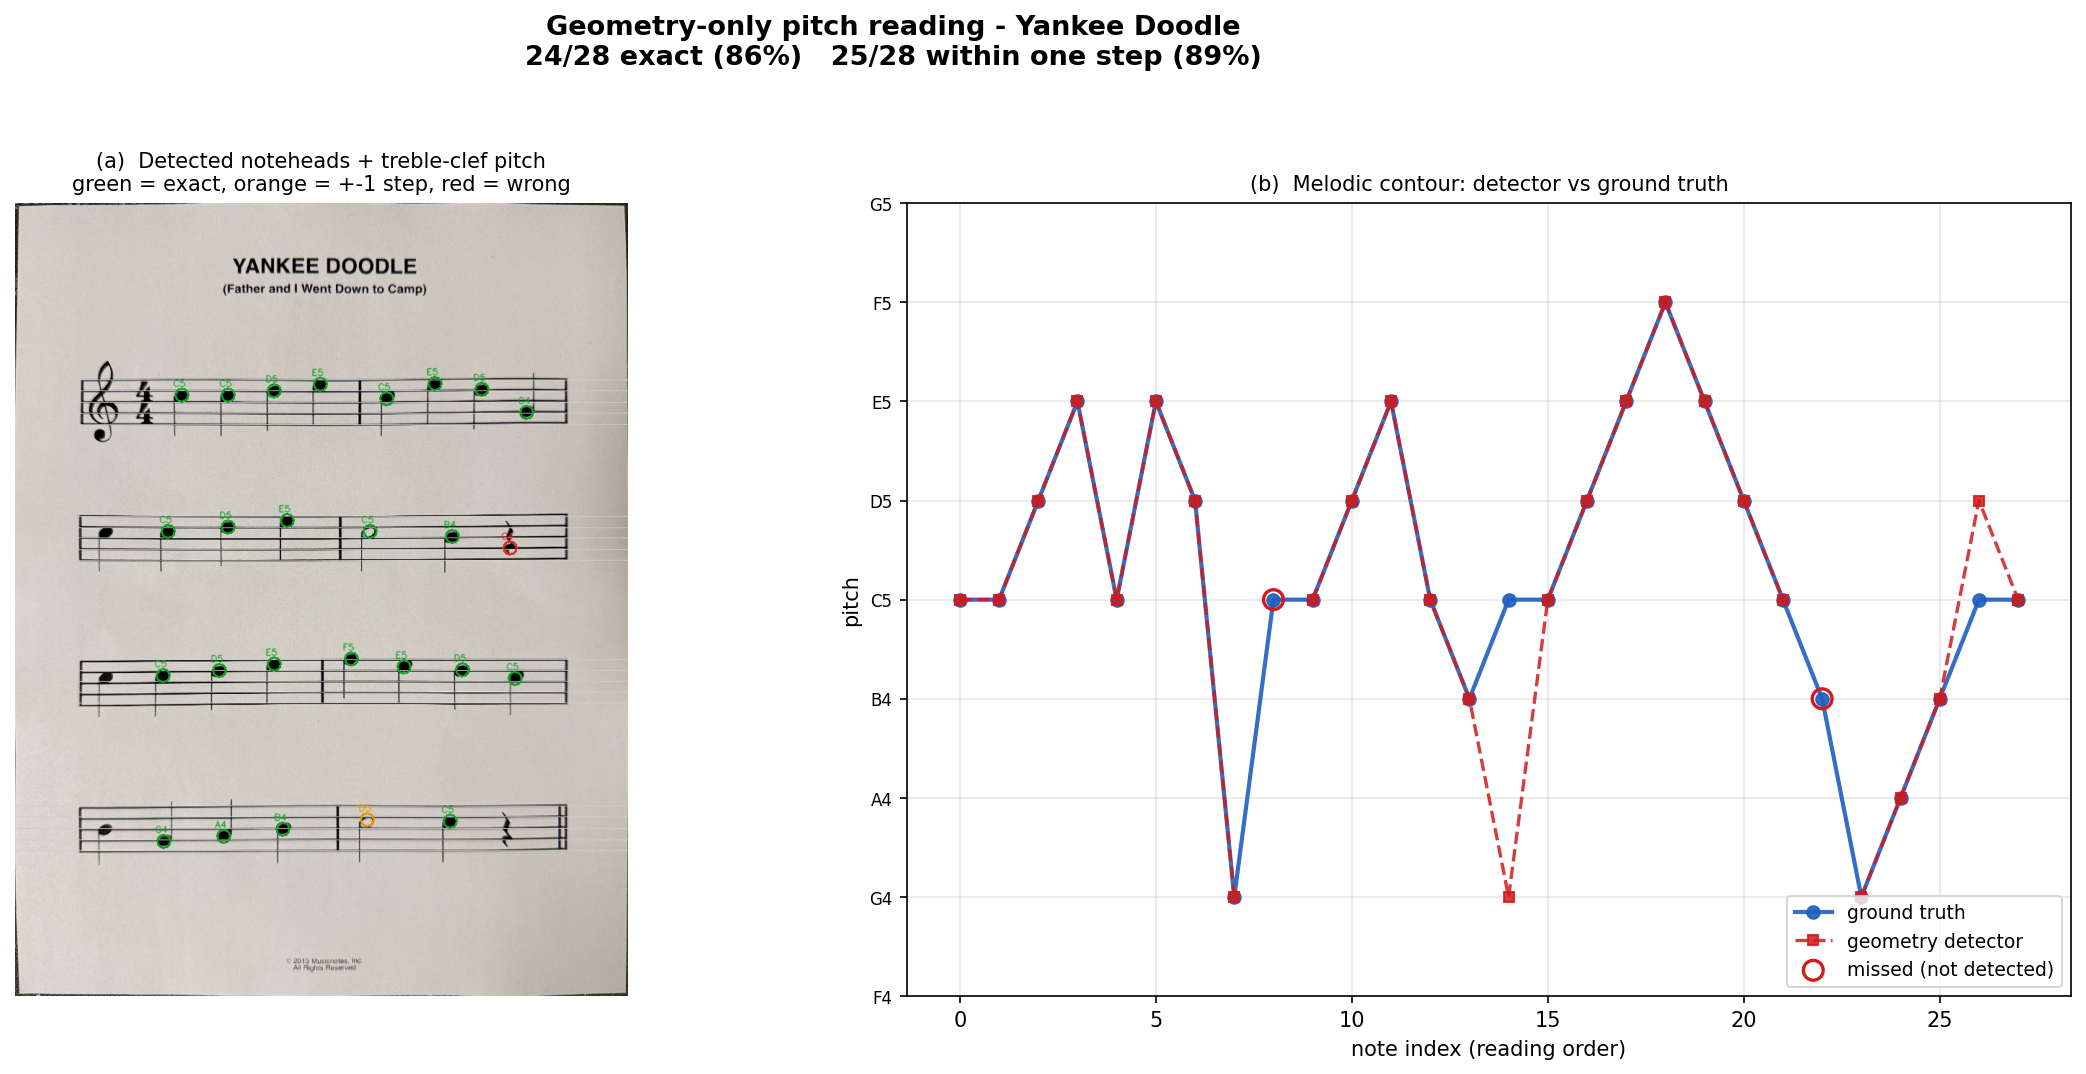
\includegraphics[width=0.44\linewidth]{figures/geometry_pitch.png}
  \caption{\textbf{Geometry-only pitch reading on \emph{Yankee Doodle}}
  (Sec.~\ref{sec:results:pitch}). Left: template-matched noteheads labelled with
  the inferred pitch (green $=$ exact, orange $=$ within one step, red $=$ wrong).
  Right: inferred melodic contour vs.\ ground truth (open circles mark the two
  undetected noteheads). The reader attains $24/28$ ($86\%$) exact and $25/28$
  ($89\%$) within one step, with no segmentation or classification.}
  \label{fig:geom_pitch}
\end{figure*}

\subsection{The clean-to-real domain gap}
\label{sec:results:gap}
The learned classifier behaves very differently on clean PrIMuS and real
photographic crops. It achieves $58.9\%$ validation accuracy on clean PrIMuS
glyphs but only $22.7\%$ accuracy on $97$ real photographic crops, a
$36.2$-point gap (Table~\ref{tab:cnn}). Class-dependent error rates reveal the
gap's scale: quarter notes are fairly robust ($24.6\%$) and eighth notes very
robust ($80\%$), but hollow half notes fail completely ($0/7$) and the residual
\emph{other} category never recovers ($0/21$). The cause is immediately apparent
from the real photo crops: the clean PrIMuS glyphs are crisp and uniform, whereas
photographic crops have blur, fractured stems, filled-in noteheads, and trace
background staff lines which the clean-trained features simply never encountered.
This is the primary insight of the paper: a system trained for appearance-based
classification on engravings does not transfer to phone photographs.

\begin{table}[t]
  \centering
  \small
  \setlength{\tabcolsep}{6pt}
  \begin{tabular}{lcc}
    \toprule
    Setting / Class & Crops & Accuracy\\
    \midrule
    PrIMuS validation (clean) & --- & $\mathbf{58.9\%}$\\
    Local phone crops (real)  & 97  & $\mathbf{22.7\%}$\\
    \midrule
    \quad note\_quarter & 57 & $24.6\%$\\
    \quad note\_eighth  & 10 & $80.0\%$\\
    \quad note\_half    & 7  & $0.0\%$\\
    \quad rest\_quarter & 2  & $0.0\%$\\
    \quad other         & 21 & $0.0\%$\\
    \midrule
    \emph{Clean-to-real gap} & & $\mathbf{-36.2}$ pts\\
    \bottomrule
  \end{tabular}
  \caption{Domain-gap study for \textsc{SymbolCNN}. A model close to $60\%$ on
  clean glyphs plunges to under $23\%$ on real-photo crops, missing its hollow and
  catch-all classes entirely.}
  \label{tab:cnn}
\end{table}

\subsection{End-to-end pitch and the geometry remedy}
\label{sec:results:pitch}
The domain gap also extends to the full pipeline. On the
segmentation-plus-classifier path, end-to-end pitch accuracy on all four pieces
is low (Table~\ref{tab:pitch}): $8$--$14\%$ exact and $17$--$50\%$ within one
step. Mistakes are due not so much to the pitch geometry of
Eq.~\eqref{eq:staffpos}---exact where the notehead is properly located---as to
upstream segmentation merges and misclassifications.

\begin{table}[t]
  \centering
  \small
  \setlength{\tabcolsep}{5pt}
  \resizebox{\columnwidth}{!}{%
  \begin{tabular}{lcccc}
    \toprule
    & \multicolumn{2}{c}{Baseline (seg.+CNN)} & \multicolumn{2}{c}{Geometry-only}\\
    \cmidrule(lr){2-3}\cmidrule(lr){4-5}
    Image & Exact & $\pm1$ & Exact & $\pm1$\\
    \midrule
    Yankee Doodle   & $14\%$ & $50\%$ & $\mathbf{86\%}$ & $\mathbf{89\%}$\\
    Twinkle Twinkle & $10\%$ & $19\%$ & --- & ---\\
    Mary Had a Lamb & $8\%$  & $23\%$ & --- & ---\\
    CS\,131 motif   & $8\%$  & $17\%$ & --- & ---\\
    \bottomrule
  \end{tabular}}
  \caption{End-to-end pitch accuracy. The seg.+CNN baseline is weak; the geometry
  reader (Sec.~\ref{sec:method:pitch}) lifts \emph{Yankee Doodle} from $14\%$ to
  $86\%$.}
  \label{tab:pitch}
\end{table}

The geometry-only reader presents a different scenario
(Fig.~\ref{fig:geom_pitch}). On \emph{Yankee Doodle} it localizes $26$ of the
$28$ noteheads and, under the standard alignment-based metric, reads $24/28$
($86\%$) pitches exactly and $25/28$ ($89\%$) within one step (a six-fold
increase over baseline). Since pitch is extracted directly from the notehead
position using Eq.~\eqref{eq:staffpos}, it is read perfectly whenever the
notehead is detected, and only two pitch-reading errors (one missed notehead pair
and one localization slip) are produced. For phone-photo OMR, geometry
generalizes where the appearance-based models trained on clean data fail.

\subsection{Diagnostics and Limitations}
\label{sec:results:limits}
It was particularly interesting to see how two approaches---overzealous
stem-bridging and over-segmentation of a glyph---resulted in failing to connect
beamed notes or completely separating a glyph. By linking the morphological
kernel size to $s$, I eliminated these problems. Another clear limit is
\emph{London Bridge}: a thick dark shadow heavily skews the page mask, so the
corner cascade returns a slanted rather than square quadrilateral, in turn
causing staff detection to fail. This highlights shadow-tolerant binarization as
future work.

\section{Conclusion and Future Work}
\label{sec:conclusion}

I proposed a five-stage phone-photo-to-MIDI pipeline called
\emph{antiTranscription}, and applied it to measure where OMR fails under actual
capture conditions. I found that geometry-based pipeline components (rectification
and Hough staff detection) transfer perfectly to phone photos, whereas an
appearance-based classifier trained on pristine PrIMuS glyphs declines in
accuracy by $36.2$ points ($58.9\%\!\rightarrow\!22.7\%$) on real captures and
fails for thin and hollow glyphs. Treating pitch detection as geometry-based
detection, as opposed to segmentation and classification, increases exact
accuracy on an exemplar piece from $14\%$ to $86\%$. I plan to address the
training gap through synthetic camera distortions (Camera-PrIMuS) and/or
feature-level adaptation~\cite{ganin2015dann}, and to generalize the
geometry-only reader to a full transcriber (including duration, accidentals, key
and time signatures, and polyphony).

\paragraph{Individual contributions.} Yameen Sekandari completed all five stages
of the pipeline, classifier training, the domain-gap experiment, and the
geometry-only reader, and wrote this paper.


{
    \small
    \bibliographystyle{ieeenat_fullname}
    \bibliography{main}
}

\end{document}
